\section{Geräteaufbau}

\subsection{Blockschaltbild der Hardware}

Durch das Blockschaltbild werden übersichtlich die Zusammenhänge der Hardware dargestellt. Es kann herausgelesen werden, dass Sensoren in die SPS führen und von der SPS Motoren und Lichter angesteuert werden.

\begin{figure}[H]
    \centering
    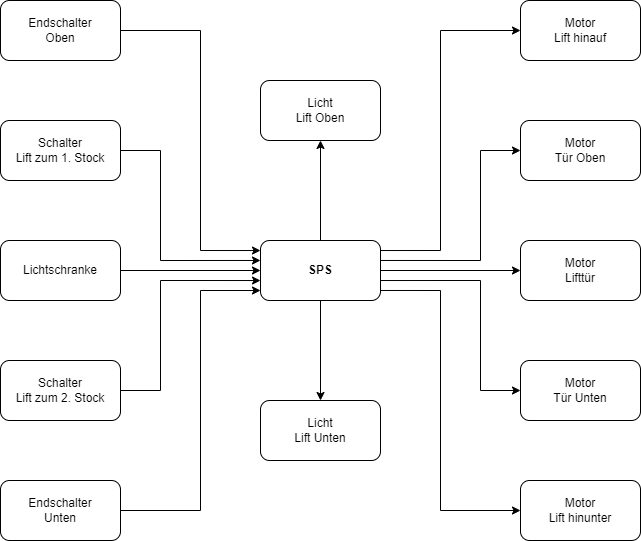
\includegraphics[width=\textwidth]{./images/Blockschaltbild.png}
    \caption[Blockschaltbild]{Blockschaltbild}
\end{figure}

Es ist wichtig die elektromagnetische Verträglichkeit zu beachten, um Falschsignale von Sensoren zu vermeiden, welche in Folge zu Sicherheitsrisiken führen könnten.

\newpage

\subsection{Struktogramm der Software}

Um den Code zu veranschaulichen, wurde ein Zustandsdiagramm entworfen.

\begin{figure}[H]
    \centering
    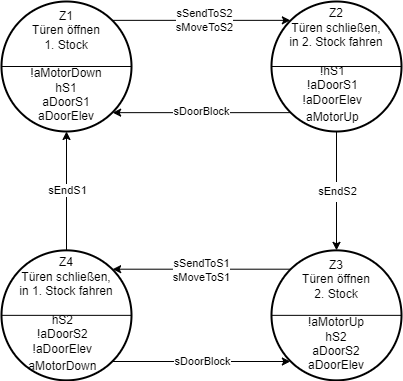
\includegraphics[width=0.5\textwidth]{./images/Zustandsdiagramm.png}
    \caption[Zustandsdiagramm]{Zustandsdiagramm}
\end{figure}